\documentclass[aps,letterpaper,11pt]{revtex4}

\usepackage{graphicx}
\usepackage{float}
\usepackage{verbatim}
\usepackage{amsmath}
\usepackage{amssymb}

\newcommand{\labno}{2}
\newcommand{\labtitle}{Analyzing Velocity and Acceleration Graphs Using Logger Pro}
\newcommand{\authorname}{Kevin Truong}
\newcommand{\professor}{Dr. Melanie Lutz}
\newcommand{\classno}{Physics 006}
\newcommand{\labpartners}{Sean Casey, Kevin Castillo, and Dulce Payan}
\newcommand{\submitdate}{February 7,2017}

\begin{document}

\begin{titlepage}
\begin{center}
\hspace{-136mm}\boxed{{\Large \textsc{Lab No. \labno}}}\\\vspace{30mm}
{\Large \textsc{\labtitle} \\ \vspace{4pt}}
\rule[13pt]{\textwidth}{1pt}\\ \vspace{150pt}
{\large By: \authorname \\ \vspace{10pt}}
Lab Partners: \labpartners \\
Instructor: \professor \vspace{10pt} \\
Solano Community College\\ \classno \\ \vspace{10pt}
\submitdate
\end{center}
\end{titlepage}

\section{Abstract}

Using the Logger Pro program in tandem with a sensor, we observed graphical representations of position, velocity, and acceleration produced by the cart with a fan on a "frictionless" ramp. First, we observed the cart moving away from the sensor and speeding up. Since the movement was away from the sensor in the positive x direction and speeding up, both the velocity and acceleration were positive. Then we observed the cart moving away from the sensor, but slowing down. Since the motion is still in the positive x direction from the origin, the velocity is still positive; however, since the cart was slowing down when traveling in the positive direction, the acceleration is negative and pointing towards the sensor. Next, we observed the cart moving towards the sensor and speeding up. The motion was going towards the origin, so the velocity is negative. Since the cart was speeding up while moving towards the origin, the acceleration is also negative and pointing towards the origin. Then we analyzed the cart moving towards the sensor, but slowing down. For this section, only vector diagrams were used to explain the velocity and acceleration of the cart. The velocity is negative because it's traveling towards the sensor from the positive x direction, and the acceleration is positive pointing away from the origin because the cart is slowing down while traveling towards the sensor. Finally, we observed the cart traveling away from the sensor, slowing down, and changing direction and traveling towards the sensor while speeding up. Before changing directions, the velocity was positive because the cart was traveling away from the origin, but the acceleration was negative because the cart was slowing down. At the moment the cart turns around, the velocity is zero and the acceleration is still negative. When the cart finally turns around, the velocity is negative because it's traveling towards the origin and the acceleration is still negative pointing towards the origin. When we were analyzing the cart traveling away from the origin in the positive x direction while speeding up, we also estimated and calculated average acceleration. Using the method of ten random points, \textit{Statistics} on the Logger Pro, endpoints, and obtaining the slope in the velocity graph we estimated the average acceleration. The average acceleration we obtained from the methods:

\begin{center}
Ten random Points: 0.193$\frac{m}{s^2}$\\
\textit{Statistics} on Logger Pro: 0.189$\frac{m}{s^2}$\\
Endpoints: 0.182$\frac{m}{s^2}$\\
Slope in Velocity Graph: 0.186$\frac{m}{s^2}$
\end{center}  

\section{Introduction}

The concepts of Classical mechanics are prevalent in our everyday life. When driving to school or throwing a ball, the actions we make are governed by classical mechanics. There are various types of kinematics: one dimensional, two dimensional, three dimensional, up to nth dimensional. Increasing dimensions adds a layer of complexity compared to the dimensions below. Nevertheless, kinematics is broken down to position(x), velocity(v), and acceleration(a) in respect to an origin, in this experiment the origin will be the sensor. When an object moves from one position in space to another position in space, the object has some displacement with respect to an origin. The rate at which the displacement happens is called velocity. The rate at which the velocity changes is called acceleration. Velocity can be presented as $\frac{dx}{dt}$ which is the derivative of position with respect to time. Acceleration can be presented as $\frac{dv}{dt}$ which is the derivative of velocity with respect to time. Acceleration can also be presented as the change in the change in position in respect to time, $\frac{d^2x}{dt^2}$. Graphically, the slope of the position vs. time graph at a specific time indicates the value of the velocity at the specific time. Likewise, the slope of the velocity vs. time graph at a specific time indicates the value of the acceleration at the specific time. Velocity and acceleration can also be represented by vectors, since velocity and acceleration are just vector quantities. Calculating the acceleration vector when given velocity vectors utilizes vector addition or subtraction. $\vec{a} = \frac{\Delta \vec{v}}{\Delta t}$ where $\Delta \vec{v} = \vec{v_1} - \vec{v_0}$, the equation states that the velocity vector at $t_1$ is subtracted by the velocity vector at $t_0$, or the velocity vector at $t_1$ is added by the negative velocity vector at $t_0$.

\newpage

\section{Experimental Details}

Equipment for this experiment includes a computer, Logger Pro Program and hardware, sensor, cart with a fan, and flat "frictionless" ramp. The computer was used to run the Logger Pro program and display the data collected. The Logger Pro Program and hardware were used to collect and organize data from the sensor. The sensor was used to read motion, and was the origin. The cart with the fan was used to model constant acceleration, it decreased or increased the velocity depending on the direction of the fan. The cart had a fast and a slow option to change the value of the acceleration. On fast, the cart would have a greater value for acceleration; on slow, the cart would have a decreased value for acceleration. The actual sign of the acceleration was dependent on which direction the cart was pointing. If the cart was pointing towards the sensor, the acceleration would be negative. If the cart was pointing away from the sensor the acceleration would be positive.  



\subsection{The Diagram of motion detected by sensor}

\begin{center}
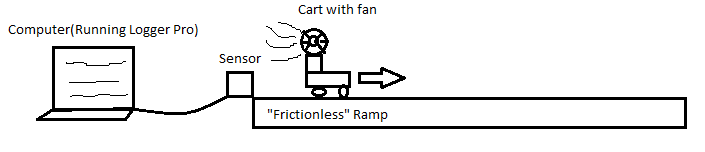
\includegraphics[width=4in]{Setup.png}
\end{center}

It's important to note that the sensor uses ultrasonic waves in a cone of 15-20$^\circ$ and will detect the closest object, so keep objects,that aren't being analyzed, away from the sensors detecting radius.  


\section{Procedures, Results and Analysis}

\subsection{Away from the Detector, and Speeding Up}

$$Speeding \hspace{1mm}up \hspace{1mm} at \hspace{1mm} a \hspace{1mm} Moderate \hspace{1mm} Rate$$

In section A, the cart was setup close to the sensor. The speed of the fan was set to low, and was released from rest. This setup models low positive constant acceleration and positive linear velocity. The positive values are due to the cart's increasing movement away from the origin. Figure 1 displays the parabolic shape of the distance vs. time graph that was the result of increasing velocity over time, this means that the distance that the cart travels over a certain interval of time, known as velocity, is increasing. If velocity was constant the distance vs. time graph would have been a linear line either pointing upward or downward depending on the direction of the movement in respect to the origin. 

\begin{center}
Figure 1\\
\vspace{-10mm}
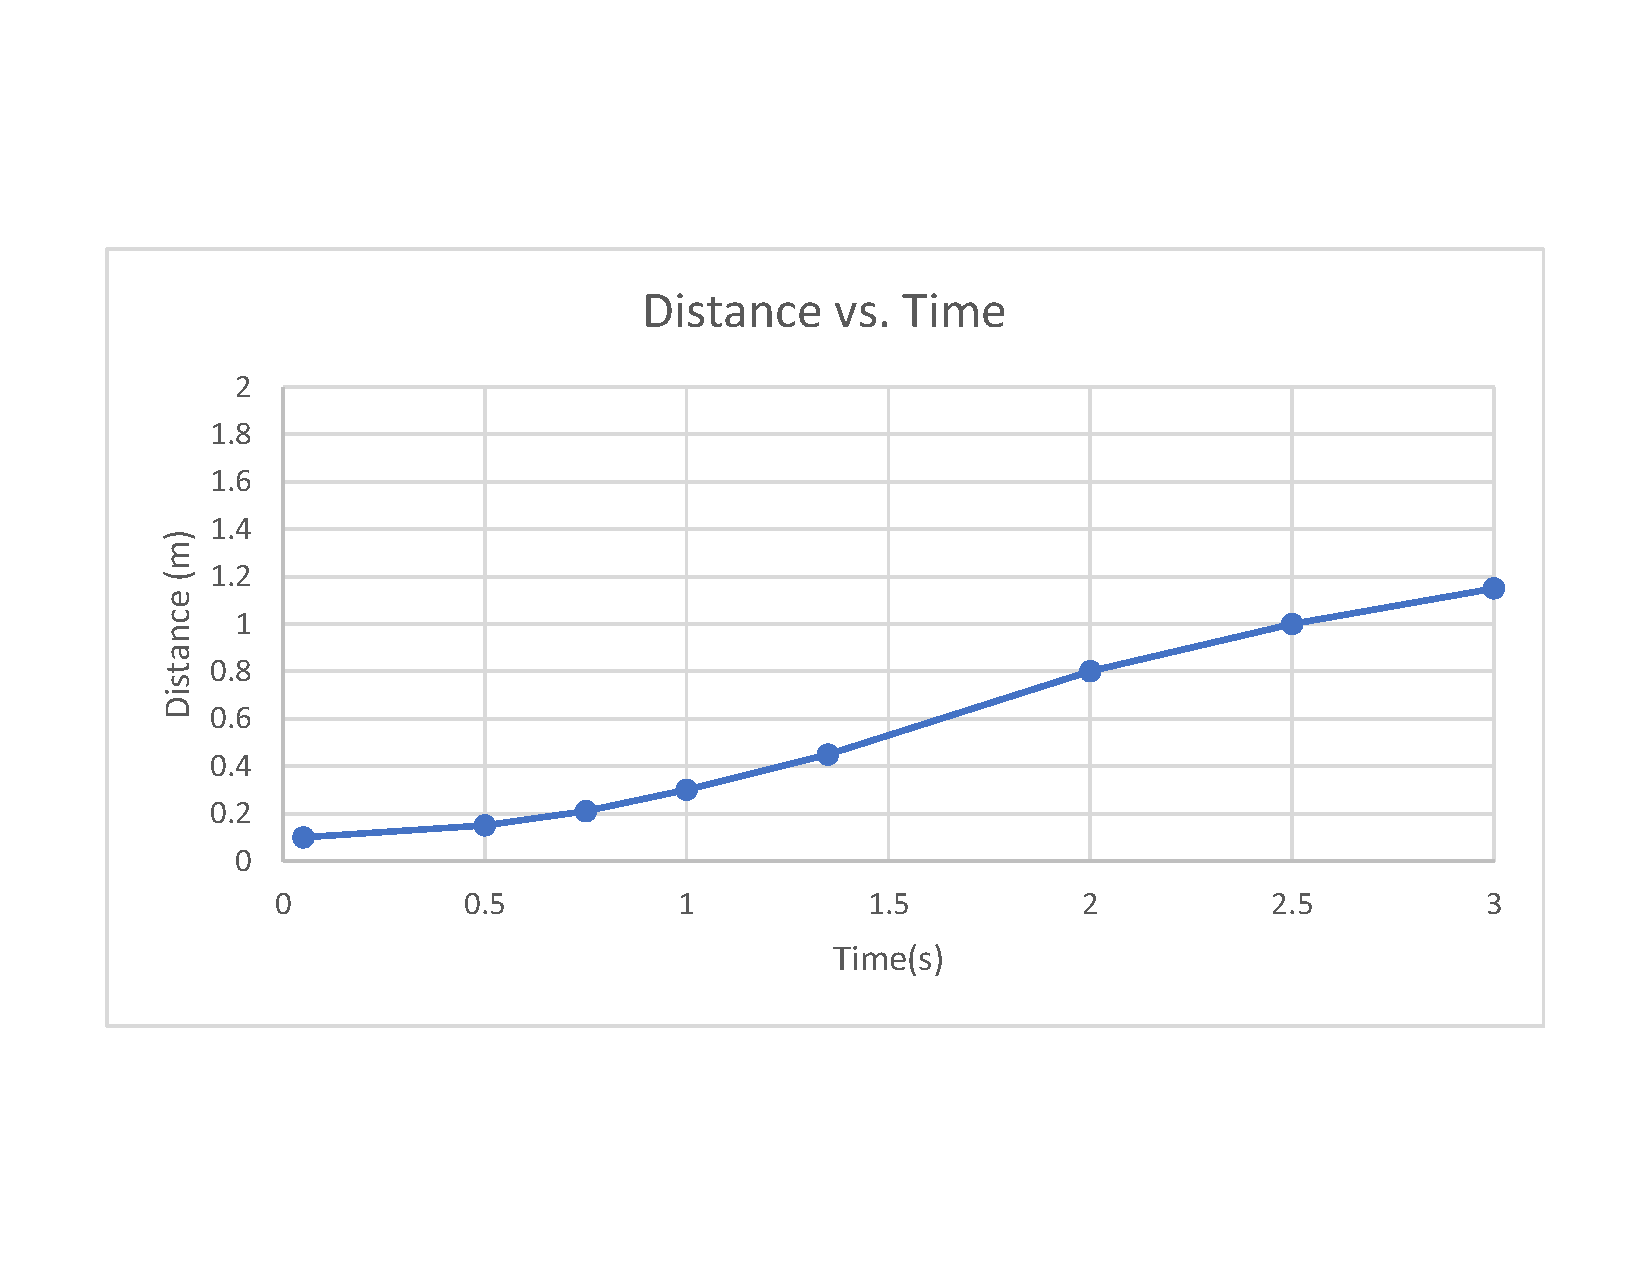
\includegraphics[width=4in]{PartADistvsTime.pdf}\\
\vspace{-10mm}
\textit{Figure 1: The distance vs. time graph for the scenario described. The parabolic shape indicates that the distance traveled was increasing over time.}
\end{center}

Figure 2 represents the velocity vs. time graph of the movement, it's a positive linear line which indicates that the velocity is increasing over time and moving away from the origin. If the velocity was constant than the velocity vs. time graph would be a horizontal line through a y-value, the specific y-value would depend on the movement of the cart in respect to the origin. 

\begin{center}
Figure 2\\
\vspace{-10mm}
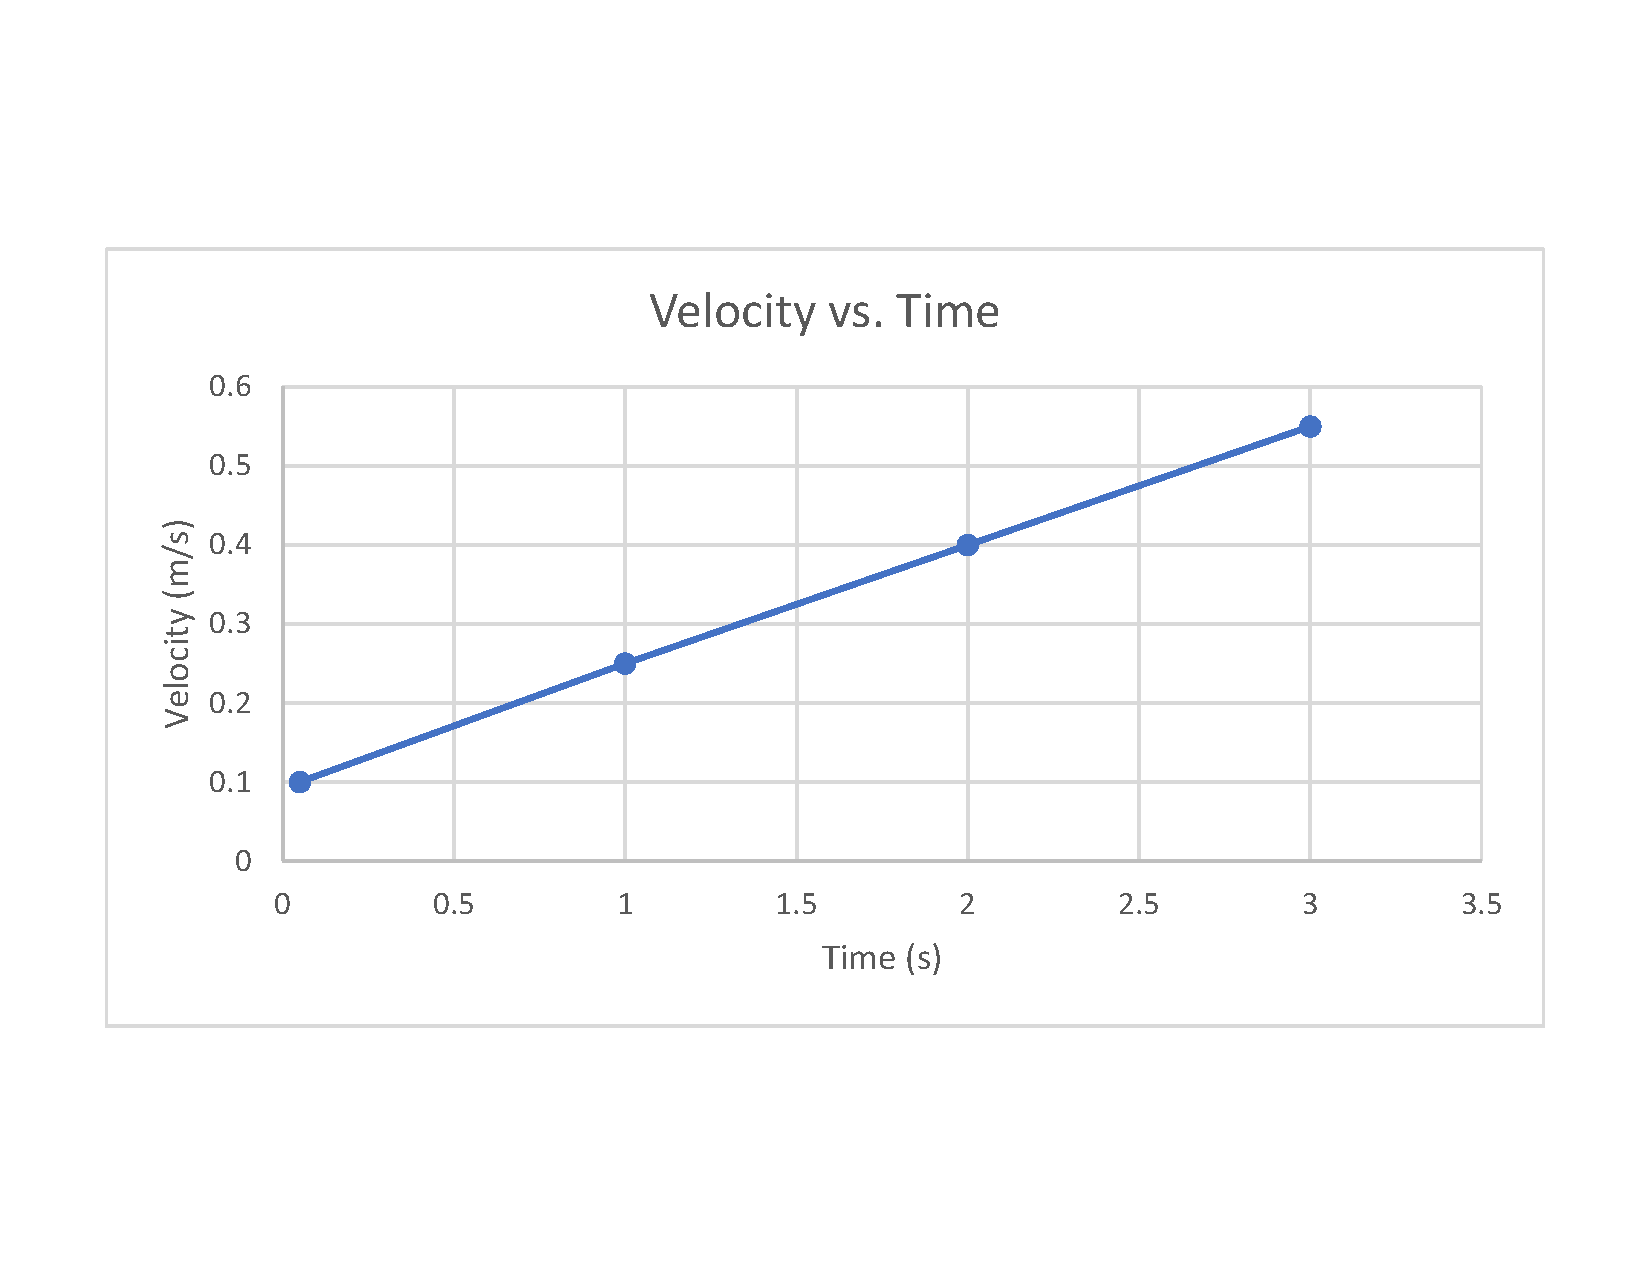
\includegraphics[width=4in]{PartAVeloctiyvsTime.pdf}\\
\vspace{-10mm}
\textit{Figure 2: The velocity vs. time graph for the scenario described. The linear positive line shows that the velocity was increasing over time while moving away from the origin.}
\end{center}
 
Analyzing the positive linear velocity, it can be predicted that the acceleration is a horizontal line through a positive y-value since velocity is increasing in the positive direction. The linear line represented in the velocity vs. time graph also means a slope that is uniform throughout the graph which indicates that the change in velocity is uniform throughout. Figure 3 models the acceleration of the system, it represents constant acceleration. The graph shows that velocity is increasing at a steady rate over an interval of time. The constant acceleration is positive because the cart was speeding up while moving away from the origin. This is supported by looking at the slope of the linear velocity line in figure 2, velocity is increasing at a constant rate and the slope is pointing in the positive direction which indicates that acceleration is positive. 
 
\begin{center}
Figure 3\\
\vspace{-10mm}
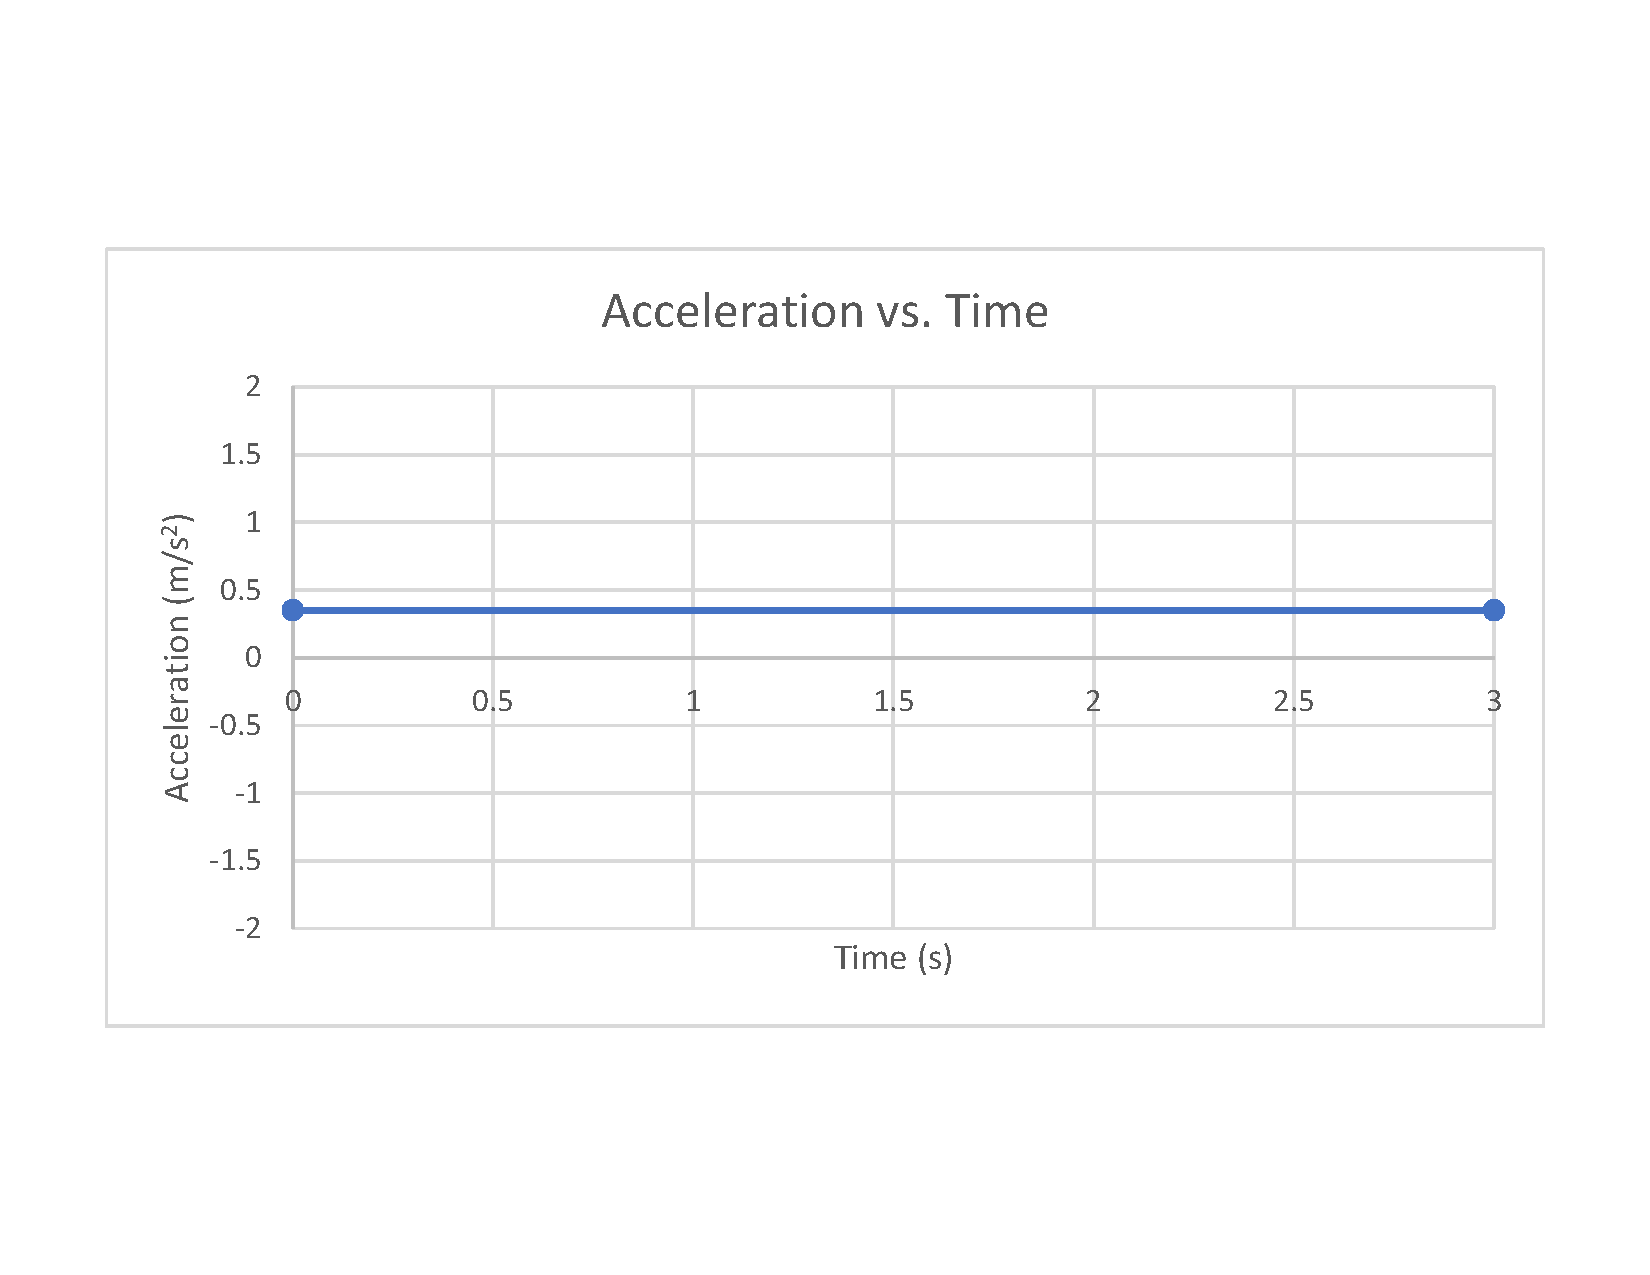
\includegraphics[width=4in]{PartAAccvsTime.pdf}\\
\vspace{-10mm}
\textit{Figure 3: The Acceleration vs. Time graph that models the rate of change of velocity in respect to time of the movement that is speeding up while moving away from the sensor}
\end{center}

\subsubsection{Using Vectors to Describe the Acceleration}

Velocity and acceleration can also be represented by vectors. Figure 4 is a diagram that shows the cart at different times and the velocity vectors at those specific times. From the diagram the velocity vector's magnitude is increasing at each interval of time, indicating that the velocity is increasing as time increases. By vector subtraction, the acceleration vector can be found from two velocity vectors. To find the acceleration vector between the times 1.0s and 2.0s, it's necessary to look at the velocity vectors $\vec{v_1}$ and $\vec{v_2}$, the acceleration vector can be found with $\vec{a} = \frac{\vec{v_2} - \vec{v_1}}{t_2 - t_1}$. Since $\vec{v_2}$ is greater than $\vec{v_1}$, $\vec{a}$ will be pointing in the positive x direction and $|\vec{a}| = ||\vec{v_2}| - |\vec{v_1}||$. In this case, the sign for acceleration would be positive because it's pointing in the positive x direction.  

\newpage
 
\begin{center}
Figure 4\\
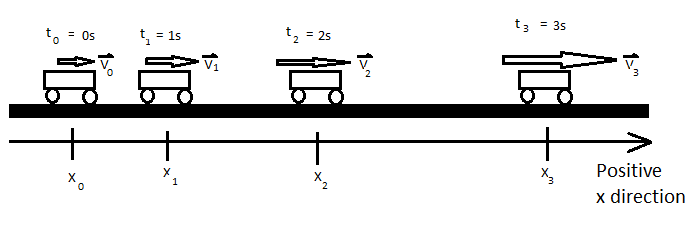
\includegraphics[width=4in]{VectorPartA.png}\\
\textit{Figure 4: Diagram that models the motion produced in part A, the velocity vectors on top of the cart show the approximate magnitude of velocity at the specific time.}
\end{center}

\subsubsection{Calculating Average Acceleration}

Three different methods were used to estimate the average acceleration of the acceleration vs. time graph(figure 3). The first method used ten random values from the bounds in the acceleration vs. time graph which we determined had constant acceleration. With the ten random values that were chosen, the average acceleration was calculated by adding up all of the values and dividing by ten.

\begin{center}
Average acceleration = 0.192$\frac{m}{s^2}$
\begin{tabular}{ |c|c|c|c| }
\hline
 & Acceleration($\frac{m}{s^2}$)\\
\hline
1 & 0.266 \\
\hline
2 & 0.209 \\
\hline
3 & 0.205 \\
\hline
4 & 0.214 \\
\hline
5 & 0.220\\
\hline
6 & 0.215\\
\hline
7 & 0.185\\
\hline
8 & 0.140\\
\hline
9 & 0.127\\
\hline
10 & 0.144\\
\hline
Total & 1.921\\
\hline
Average & 0.1921\\
\hline
\end{tabular}
\end{center}

\newpage

The second method used to find average acceleration utilized the \textit{Statistics} function in the Logger Pro program to estimate the average acceleration between the same bounds in the acceleration vs. time graph using all of the acceleration values. The Average acceleration estimated by the Logger Pro program in the bounded region was 0.189$\frac{m}{s^2}$. Between the first method and the second method used to estimate the average acceleration, they differed by 0.003$\frac{m}{s^2}$. 

The Third method used to estimate the average acceleration was finding a regression line to fit the constant acceleration portion of the velocity graph. The regression line is a linear line, so the equation that models it is in $y = Mx + b$ form. The slope($M$) of this regression line is an estimate of the average acceleration. The slope of the regression line and the estimate average acceleration was 0.186$\frac{m}{s^2}$. All of the estimated average accelerations were relatively close which is good because they agree with each other. 

We calculated the average acceleration between the same bounds in the velocity vs. time graph that was being examined. Using the equation $\bar{a} = \frac{\Delta v}{\Delta t}$, it was possible to calculate the average acceleration. 

\begin{center}
\begin{tabular}{|c|c|c|}
\hline
  & Velocity$\frac{m}{s}$ & Time(s) \\
\hline
Left end point & 0.318 & 2 \\
\hline
Right end point & 0.409 & 2.5 \\
\hline  
\end{tabular}
\end{center}

\[ \bar{a} = \frac{v_2 - v_1}{t_2 - t_1}\]

\[ \bar{a} = \frac{0.409\frac{m}{s} - 0.318\frac{m}{s}}{2.5s - 2s}\]

\[ \boxed{\bar{a} = 0.182\frac{m}{s^2}}\]

The calculation is relatively close to the estimations. The calculated value and estimations should be pretty close to each other. The difference between the calculations and estimations might be due to the small bumps that occured on the graphs. 

\subsubsection{Speeding up at a Faster Rate}

In this section the speed of the fan will be set on high. Since the movement is still going away from the origin(sensor), the veloctiy graph will still be sloped upward in the positive direction. Since the fan is on high, the slope of the velocity graph should be steeper than the slope of the velocity graph when the fan was set on low. The constant acceleration value should be a higher y-value, still positive because velocity is increasing as it moves away from the origin. Figure 5 is my prediction for the velocity and acceleration graphs when the fan is set on high compared to the actual velocity and acceleration graphs of when the fan was set on low. My predictions are the dashed lines while the actual data from the last acceleration and velocity graphs are the solid lines.

\begin{center}
Figure 5\\
\vspace{-10mm}
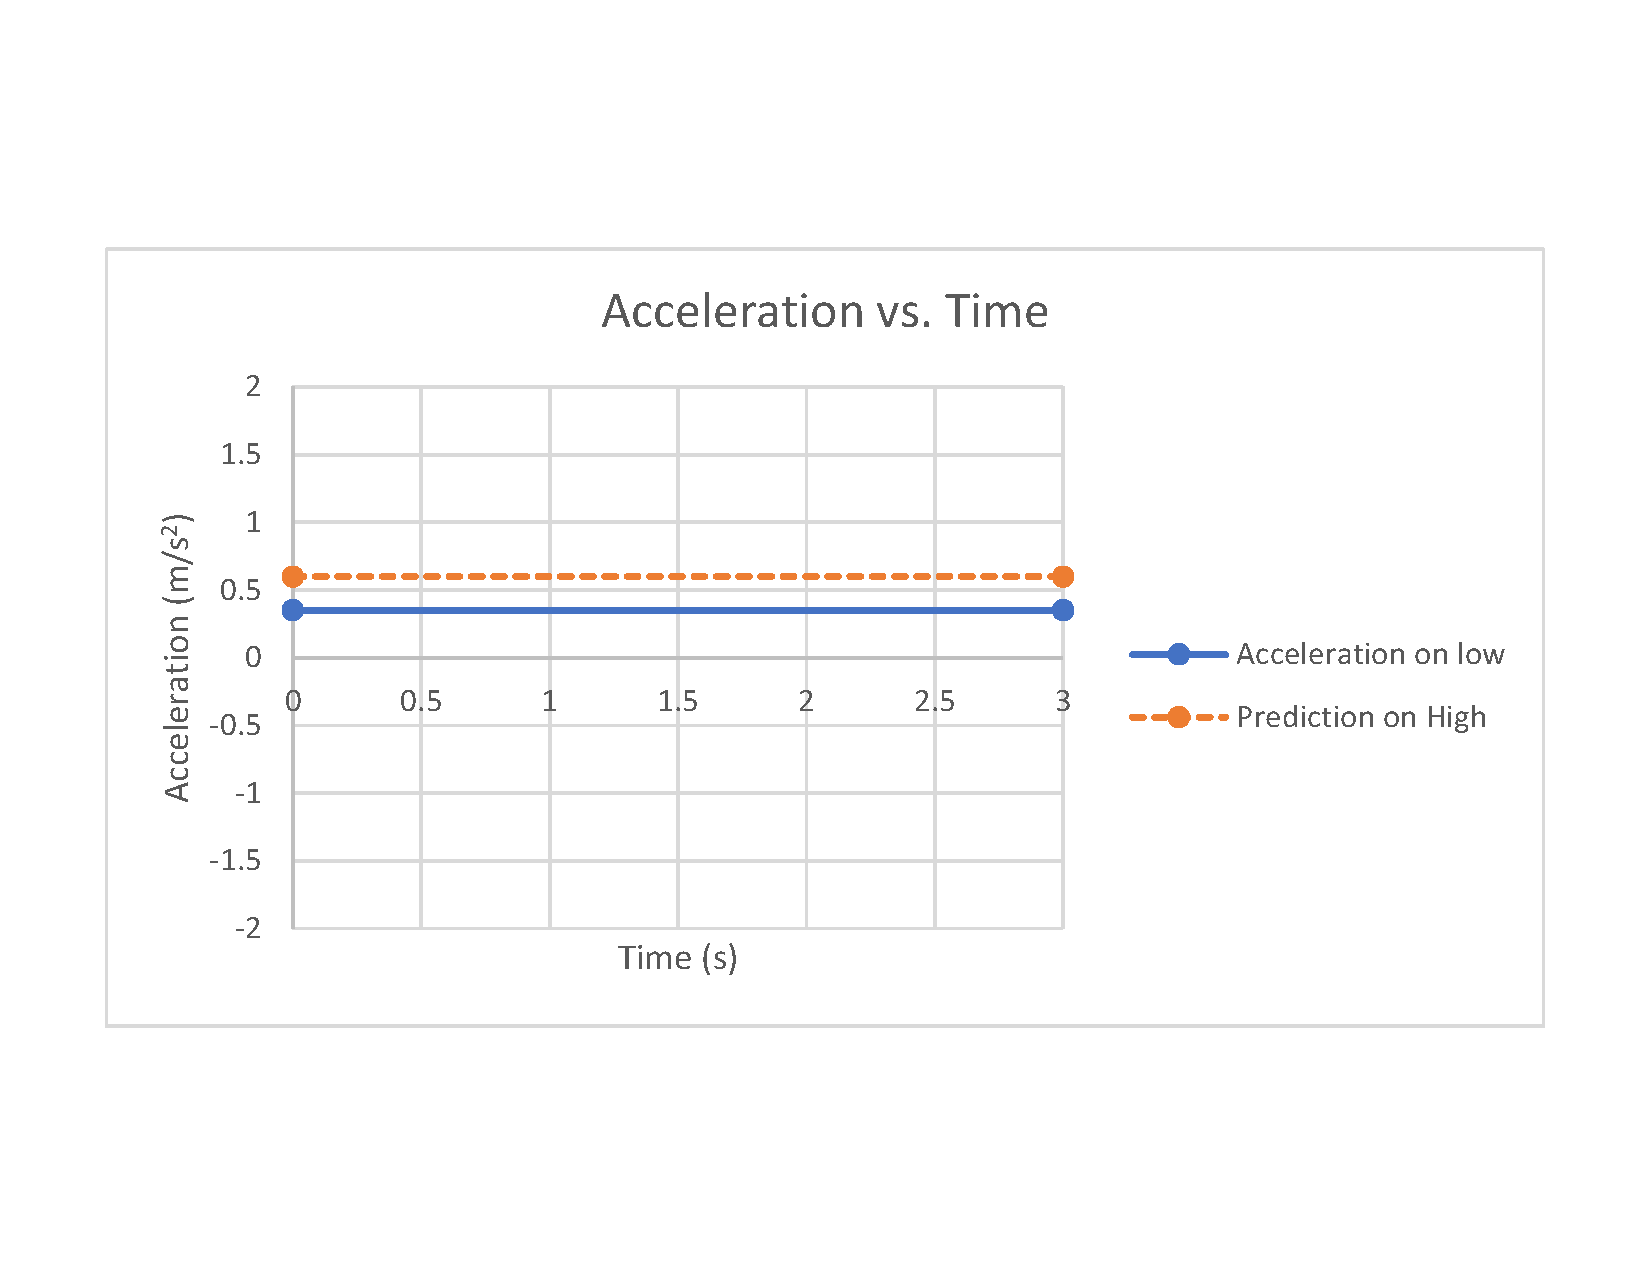
\includegraphics[width=4in]{PartAPredHighActLow.pdf}\\
\vspace{-10mm}
\textit{Figure 5a: The Acceleration vs. Time graph with the predicted acceleration with the fan set on high and the actual acceleration when the fan was set on low.}\\
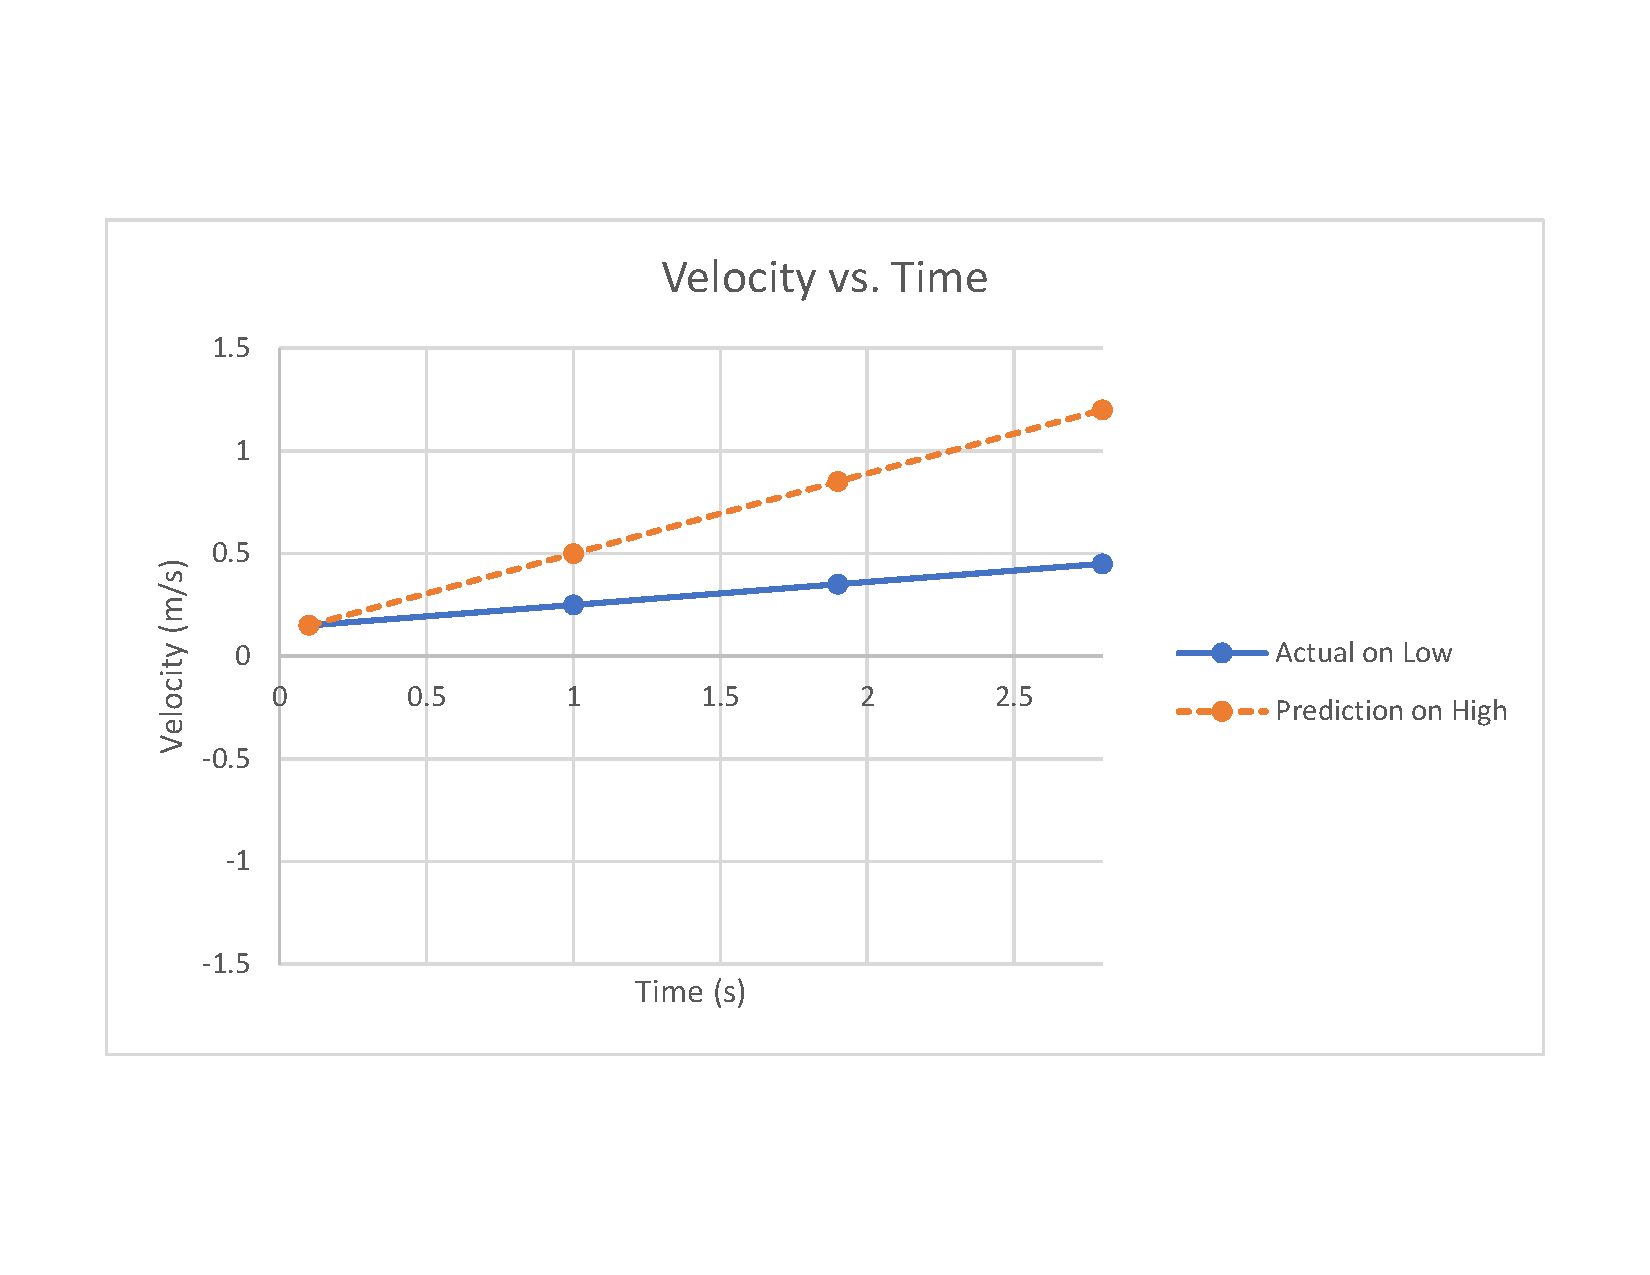
\includegraphics[width=4in]{PartAPredHighActLowVel.pdf}\\
\vspace{-10mm}
\textit{Figure 5b: The Velocity vs. Time graph with the predicted velocity with the fan set on high and the actual velocity when the fan was set on low.}
\end{center}

\newpage 

Figure 6 shows the actual acceleration vs. time graph and velocity vs. time graph that was produced from movement away from the origin while the fan was set on high.
The actual acceleration vs. time graph was exactly the same as my prediction, the acceleration doubled when the setting was changed from low to high. The velocity vs. time graph was very similar to my prediction, both graphs showed a steeper slope indicating that the velocity was increasing faster than when the fan setting was on low. 

\begin{center}
Figure 6\\
\vspace{-10mm}
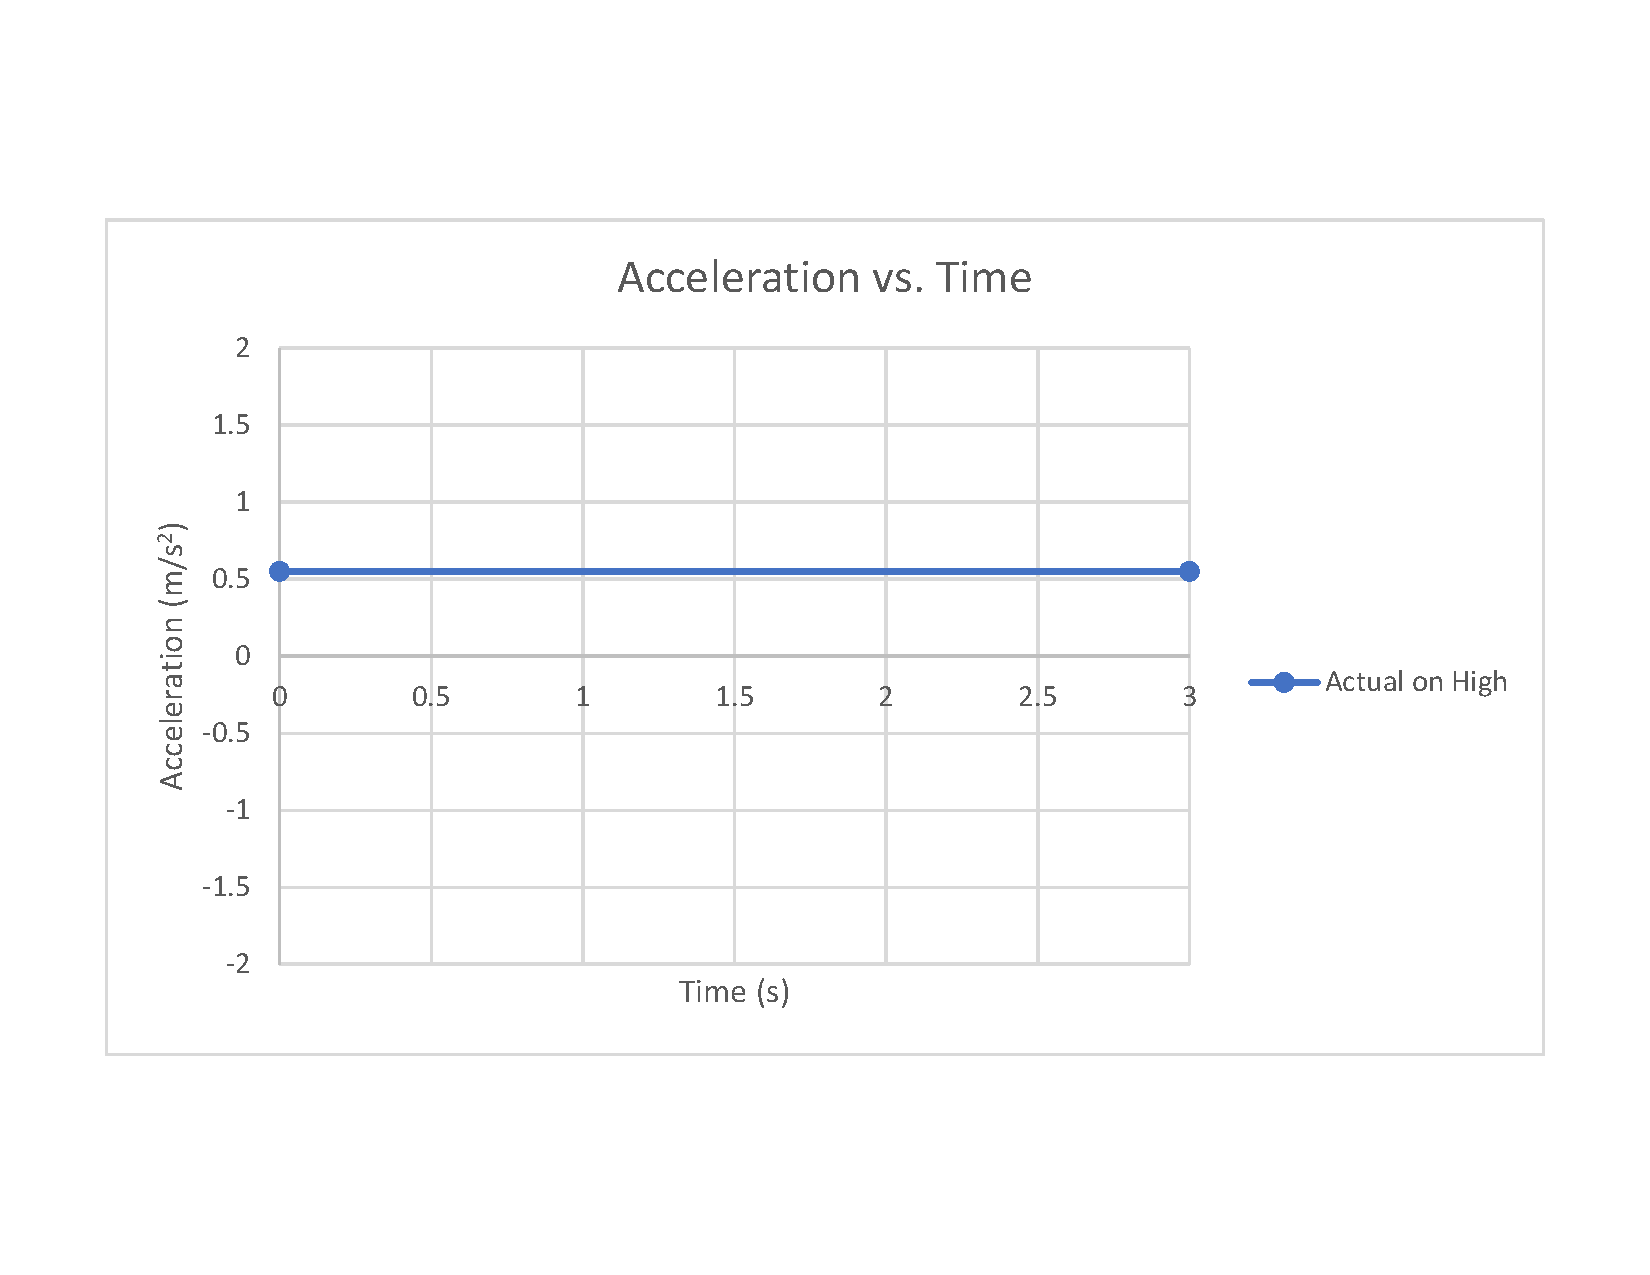
\includegraphics[width=4in]{PartAActualAcc.pdf}\\
\vspace{-10mm}
\textit{Figure 6a: The actual Acceleration vs. Time graph from the motion produced with the fan set on High}\\
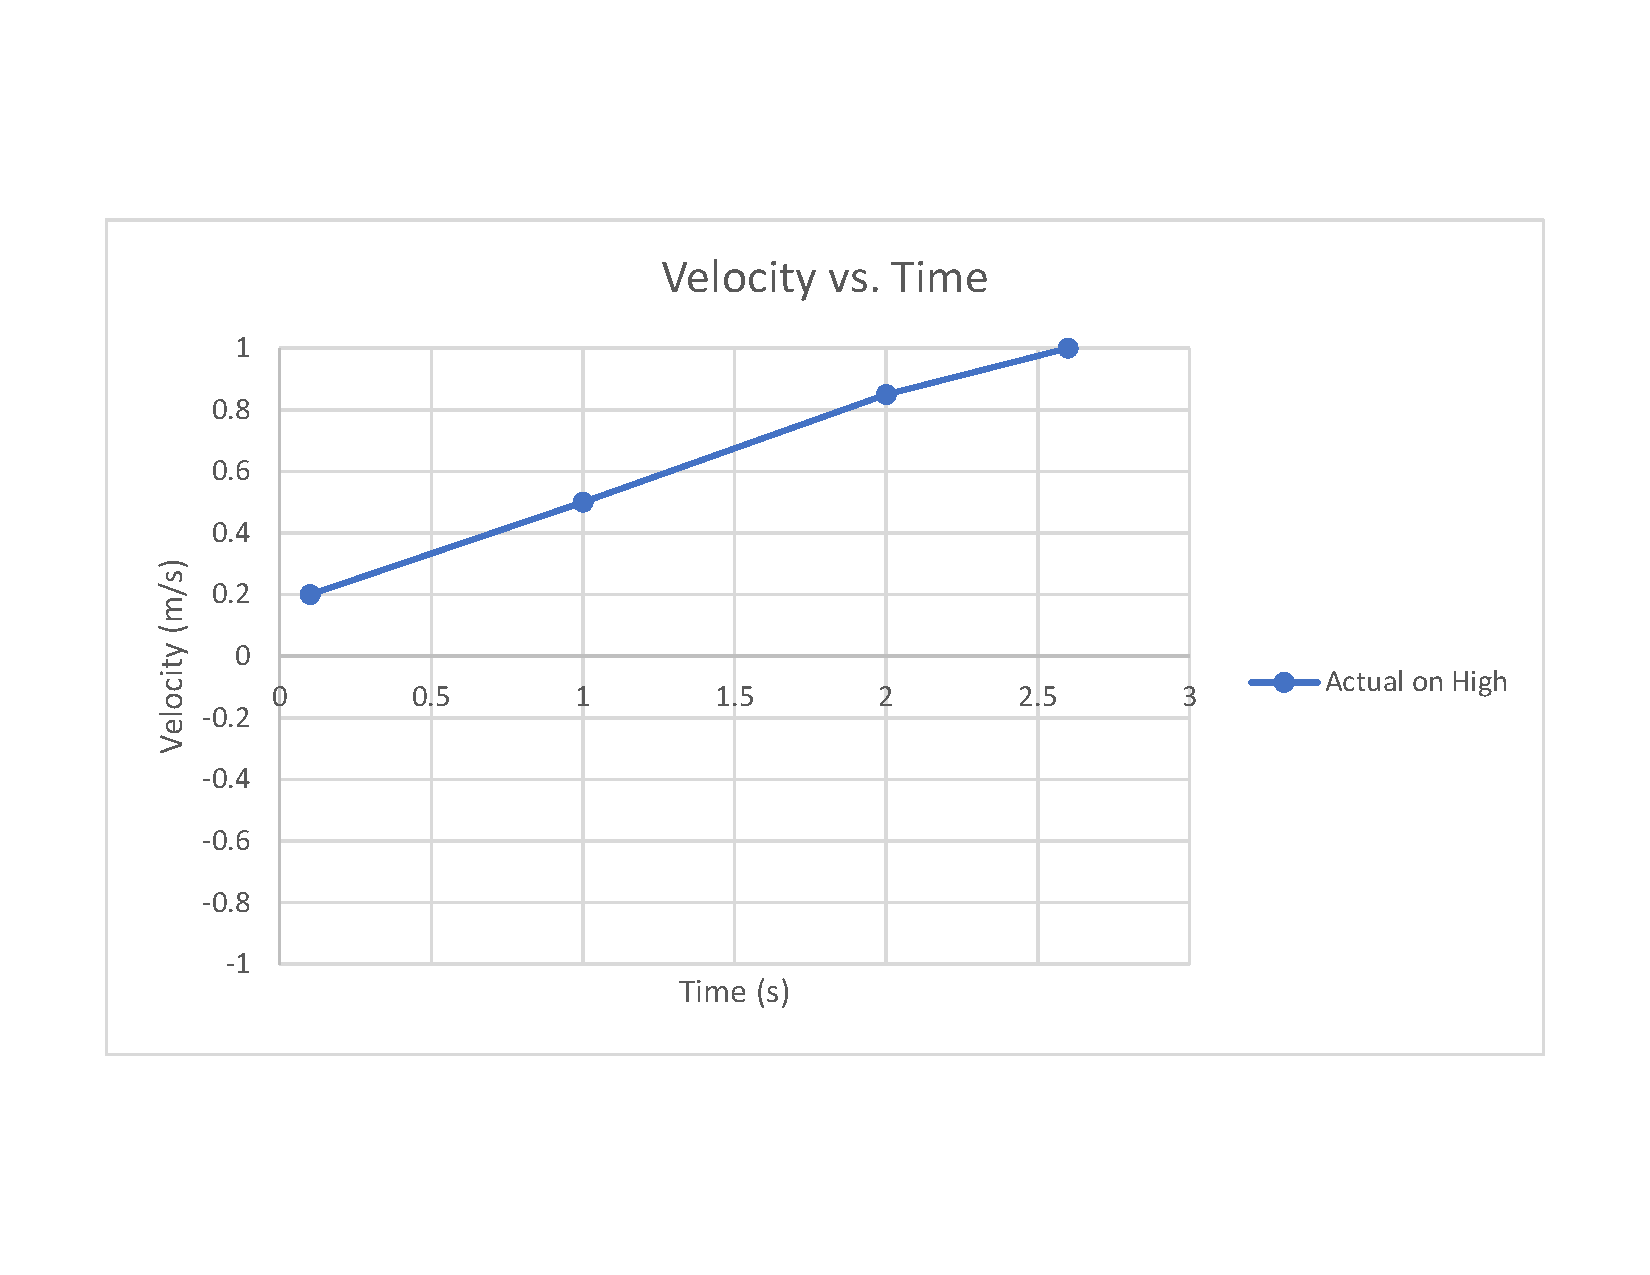
\includegraphics[width=4in]{PartAActualVel.pdf}\\
\vspace{-10mm}
\textit{Figure 6b: The actual Velocity vs. Time graph from the motion produced with the fan set on High}
\end{center}

\newpage 

The graphs show that the constant acceleration value has increased substantially from the fan being set on high compared to when the fan was set on low. Using the $Statistics$ feature on the Logger Pro program, we examined the mean acceleration when the fan was set on high. Now it is possible to compare the mean acceleration from when the fan was set on high and when the fan was set on low(found using the second method).

\vspace{10mm}

\begin{center}
\begin{tabular}{|c|c|}
\hline
  & Mean acceleration\\
\hline
Fan on high & 0.303$\frac{m}{s^2}$\\
\hline
Fan on low & 0.189$\frac{m}{s^2}$\\
\hline  
\end{tabular}
\end{center}

\vspace{10mm}

The greater magnitude of acceleration is represented in the velocity vs. time graph by the steeper slope of the linear line. The greater magnitude of acceleration is represented in acceleration vs. time graph with the horizontal line going through a greater y-value.

\vspace{10mm
}
\subsection{Away from the Detector and Slowing Down} 

In this section, the cart and fan will be pointing towards the sensor and the fan will be set on low. An initial push of the cart away from the sensor will model a system that is moving away from the sensor, but slowing down. The acceleration will be negative because the cart is slowing down while moving away from the sensor. The velocity will have an initial high velocity, but will steadily slow down until it changes directions. Figure 7 shows my prediction of what the acceleration vs. time graph and velocity vs. time graph will look like, represented by the dashed lines, when the cart is moving away from the origin but slowing down, and the actual curves that were produced from the experiment, indicated by the solid line. 

\newpage

\begin{center}
Figure 7\\
\vspace{-10mm}
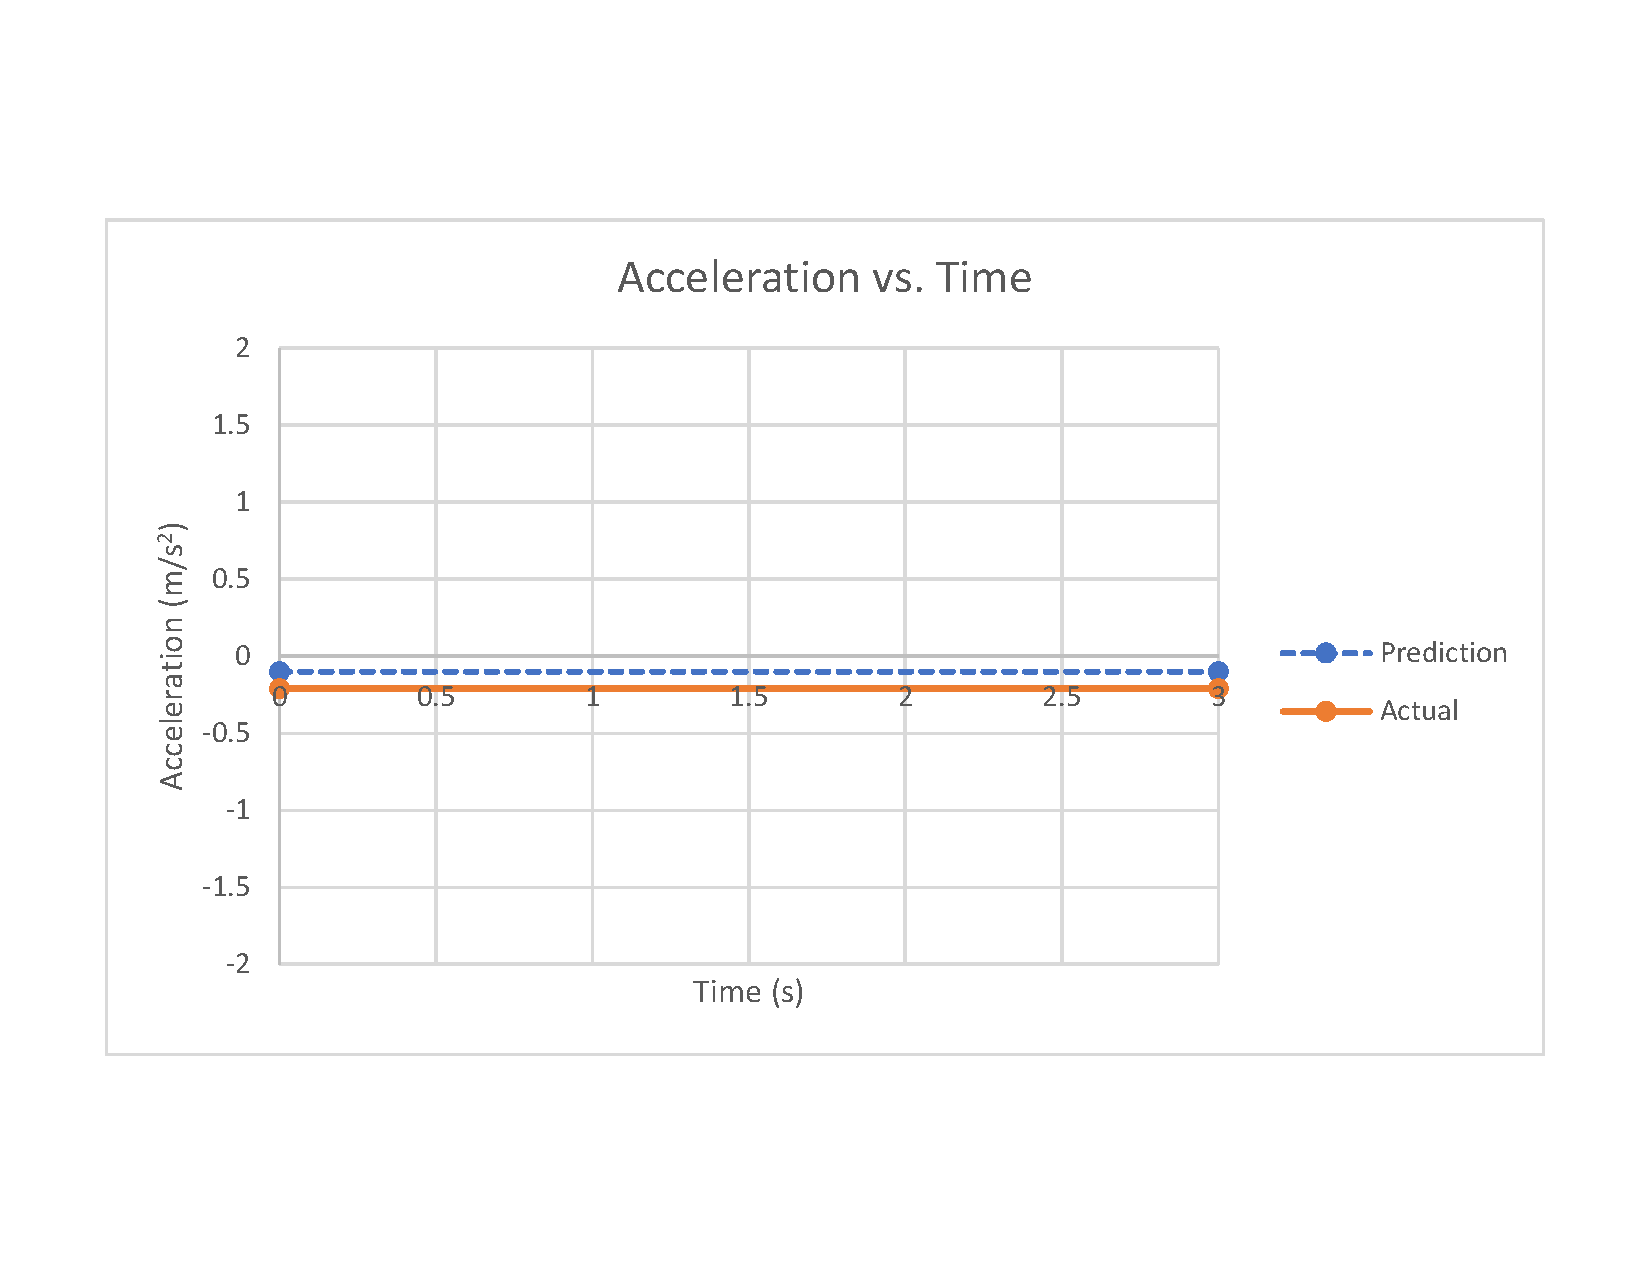
\includegraphics[width=4in]{PartBSlowingdownAcc.pdf}\\
\vspace{-10mm}
\textit{Figure 7a: The Acceleration vs. Time graph from the motion produced by slowing down while moving away from the origin. The dashed line is my prediction of the experiment, and the solid line is the actual result of the experiment.}\\
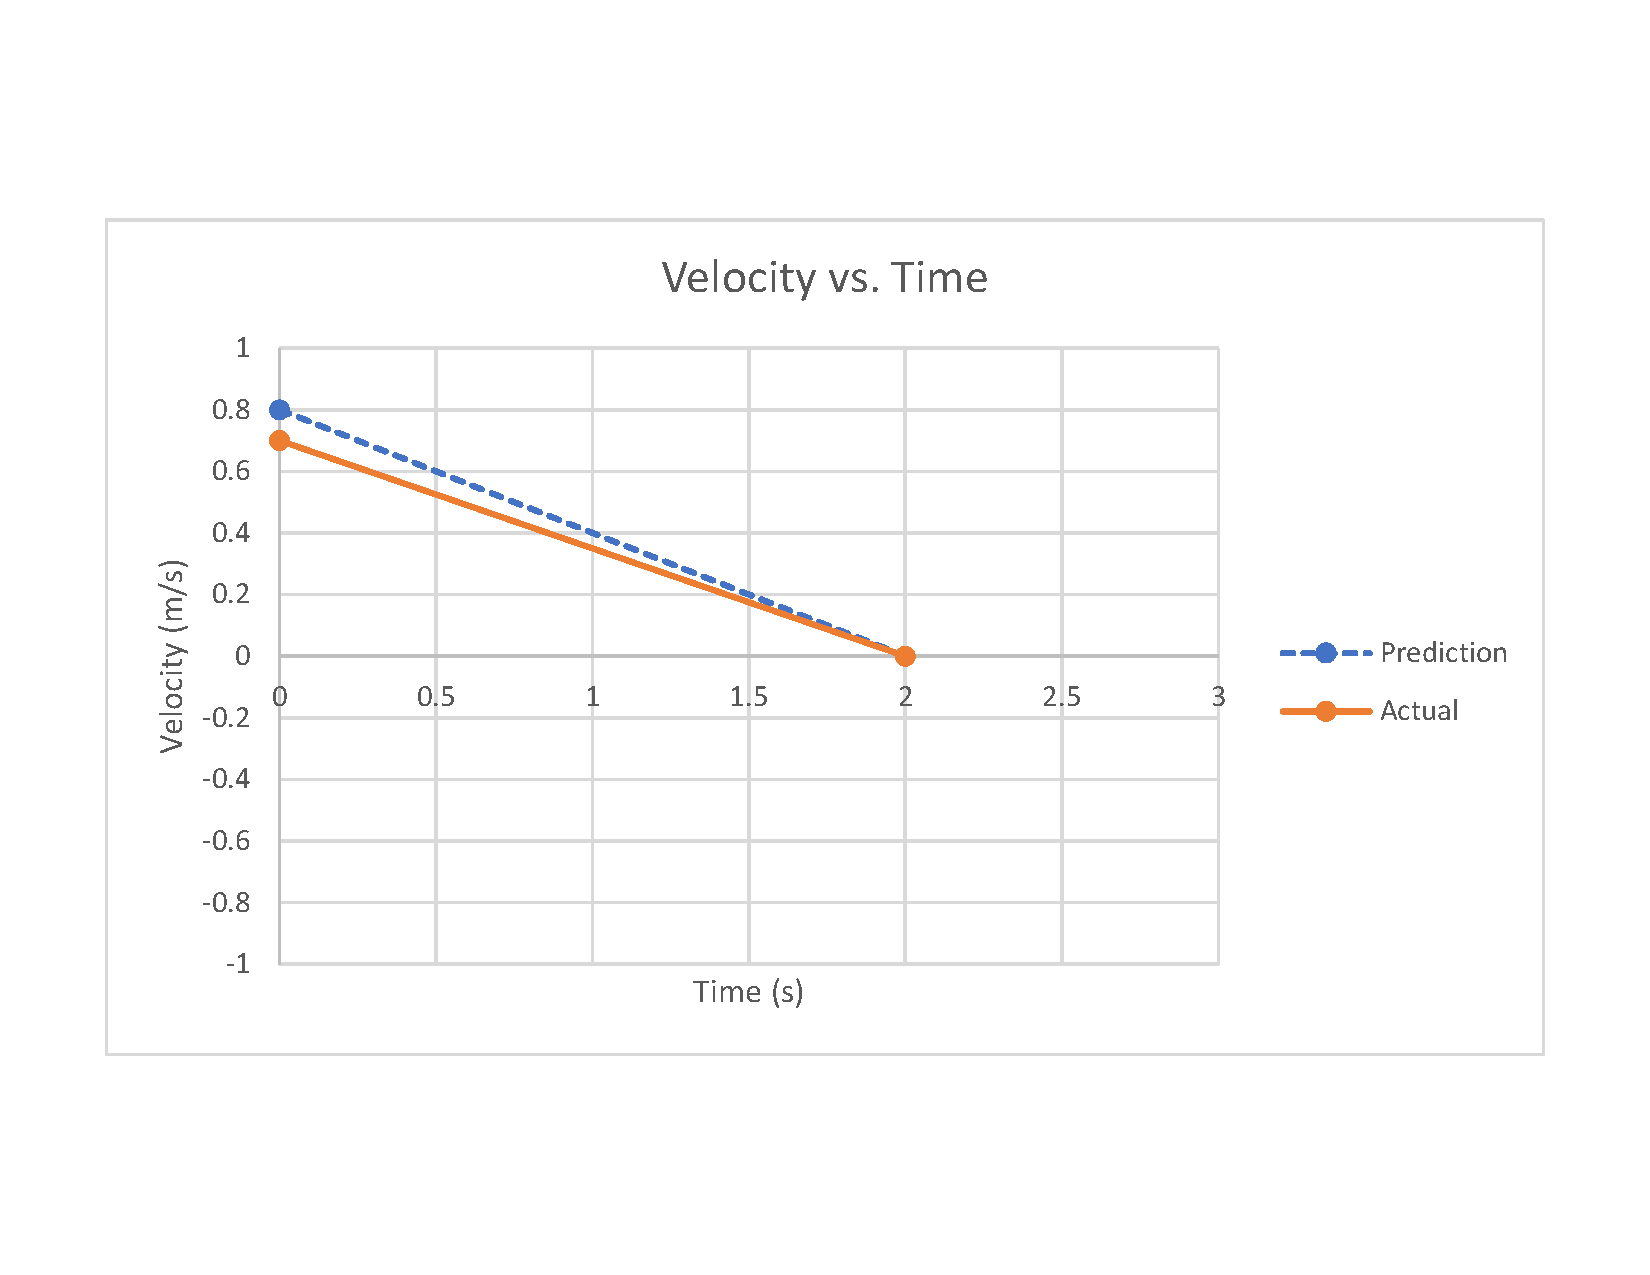
\includegraphics[width=4in]{PartBSlowingDownVel.pdf}\\
\vspace{-10mm}
\textit{Figure 7b: The Velocity vs. Time graph from the motion produced by the experiment. The dashed line is my prediction, and the solid line is the actual result of the experiment.}
\end{center}

My prediction and the actual curve from the section's experiment are very similar. However, I thought that the constant acceleration would be closer to the x-axis, the actual acceleration was a greater  negative value which explains the steeper slope in the velocity vs, time graph when compared to my prediction. Compared to the last section's experiment(Figure 6), the curves are opposite of each other. In the last section the acceleration was positive and the velocity graph was sloping upward in the positive direction. In this section's experiment the acceleration is negative and the velocity graph has a slope that is pointing downward in the negative direction. The acceleration is still constant, so the line is horiztonal through a y-value; the value is negative because the cart is slowing down while moving away from the origin which indicates that the acceleration is pointing towards the origin. The velocity is slowing down at a constant rate which is represented in the velocity vs. time graph by the negative slope.

\subsubsection{Constructing Acceleration Vectors for Slowing Down}

Just like in section A, the velocity and acceleration can also be represented by vectors. In Figure 8, the carts are moving away from the origin but are slowing down. This decrease in velocity is modeled by the decrease in magnitude of the velocity vectors. The acceleration vector between times 1s and 2s in figure 8 can be found using $\vec{a} = \frac{\vec{v_2} - \vec{v_1}}{t_2 - t_1}$. Since $|\vec{v_1}|$ is greater than $|\vec{v_2}|$, $\vec{a}$ will be negative. $\vec{a}$ is negative indicates that the vector is pointing towards the origin. The negative acceleration vector agrees with the data presented by the acceleration vs. time graphs (Figure 7). 

\begin{center}
Figure 8\\
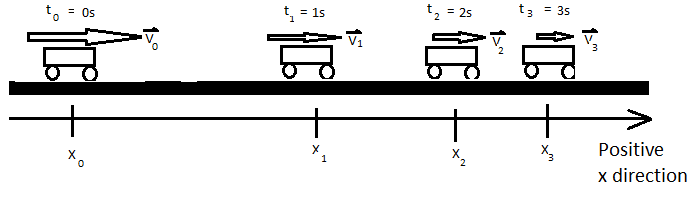
\includegraphics[width=4in]{VectorPartB.png}\\
\textit{Figure 8: Diagram that models the motion produced in part B, the velocity vectors on top of the cart show the approximate magnitude of velocity at the specific time.}
\end{center}

\subsubsection{General Rule for Predicting Sign and Direction of Acceleration}

A general rule to predict the sign and direction of the acceleration can be made when the sign of the velocity is known. The direction and sign of acceleration can be found by looking at the slope and the direction of the velocity graph. If the slope of the velocity graph is pointing downward, the acceleration is negative. If the slope of the velocity graph is pointing upward, the acceleration is positive. If the velocity vs. time graph is a linear line, the acceleration is a horizontal line through a y-value. 


\subsection{Toward the Detector and Speeding Up}

In this section the experiment that we will be conducting will have the cart and fan beginning farthest away from the origin and speeding up while moving towards the origin. It is important to stop the cart before it collides with the sensor because it will be quite fast when it gets closer to the sensor. Figure 9 shows my prediction and the actual data of what the acceleration vs. time graph looked like. My prediction(dashed line) was very similar to the actual data(solid line), but I didn't take into account that we were going to stop the cart earlier before it crashes into the sensor. In figure 9, there is also my prediction and the actual data of what the velocity vs. time graph looked like. Again my prediction was quite similar to the actual data, but I didn't take into account when we were going to stop it before it came too close to the sensor.

\begin{center}
Figure 9\\
\vspace{-10mm}
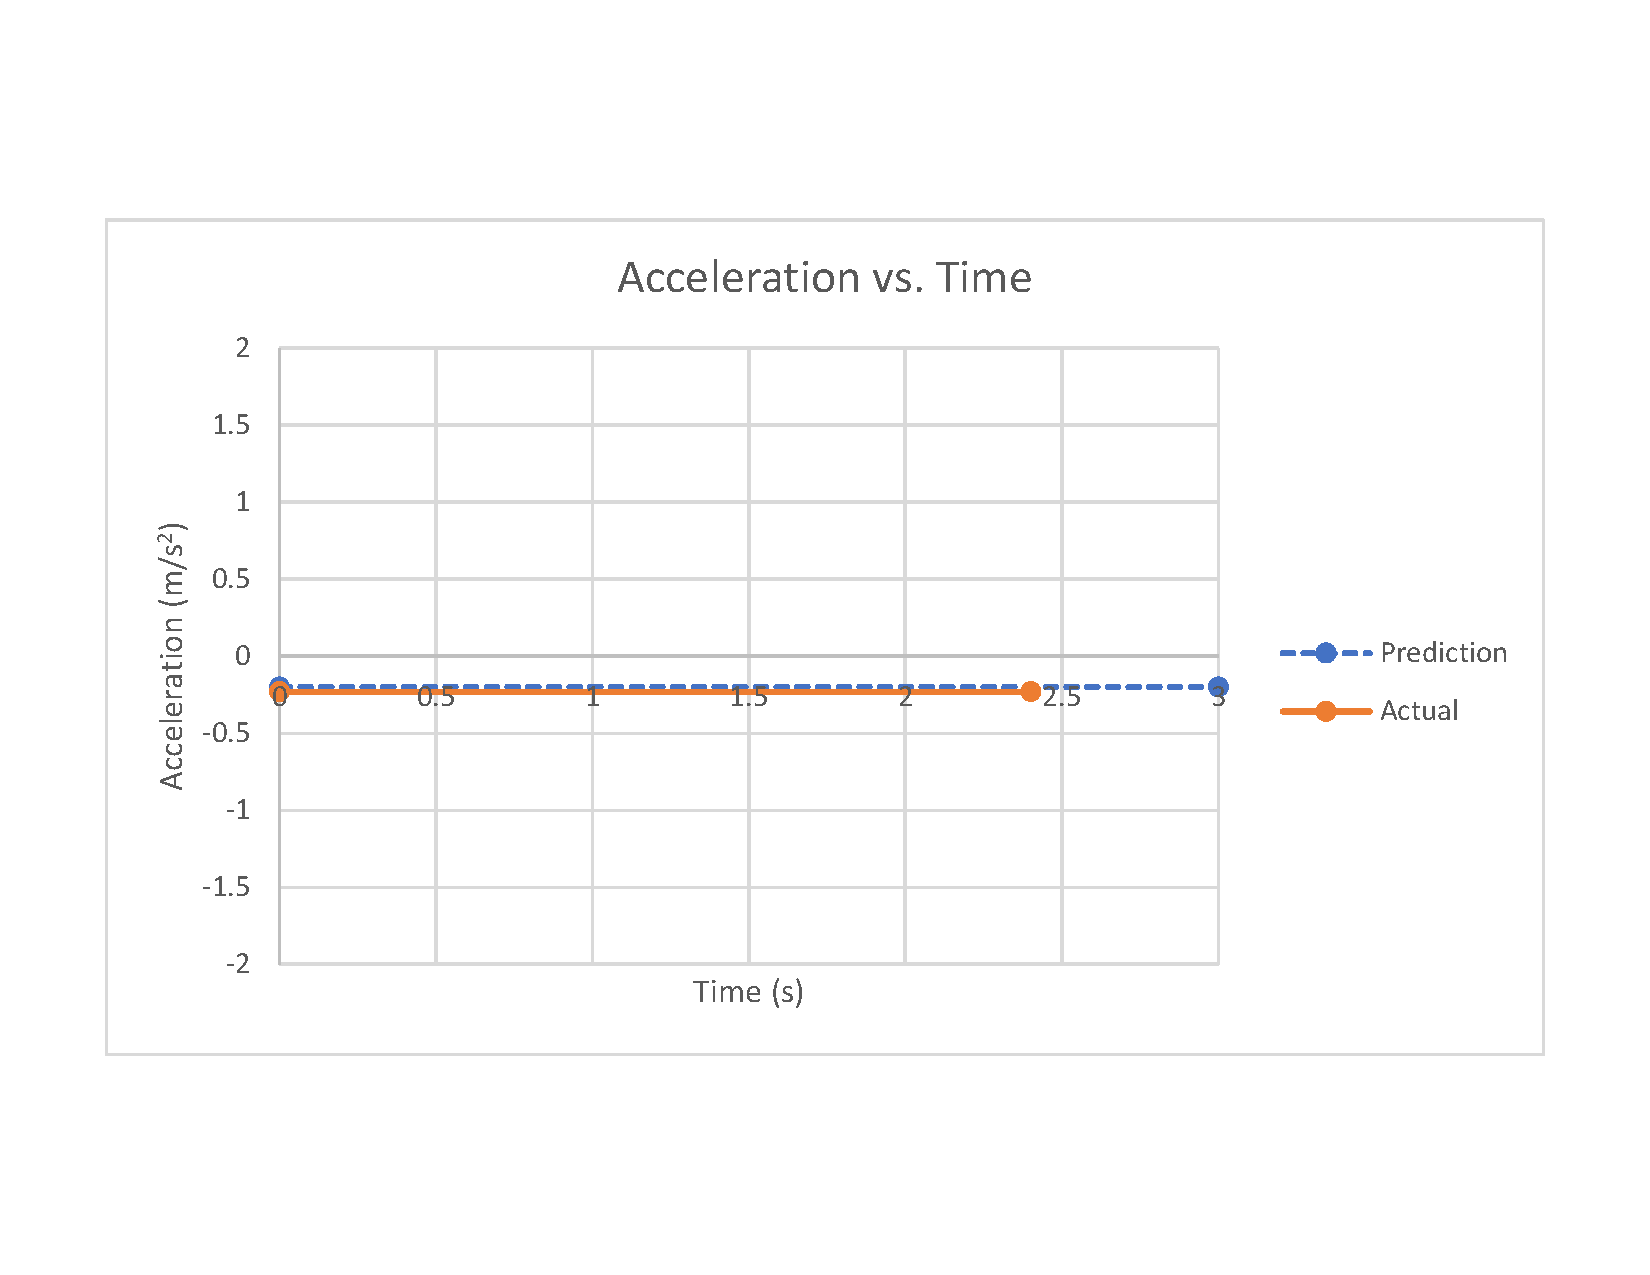
\includegraphics[width=4in]{PartCAcceleration.pdf}\\
\vspace{-10mm}
\textit{Figure 9a: The Acceleration vs. Time graph from the motion produced by speeding up while moving towards the origin. The dashed line is my prediction of the experiment, and the solid line is the actual result of the experiment.}\\
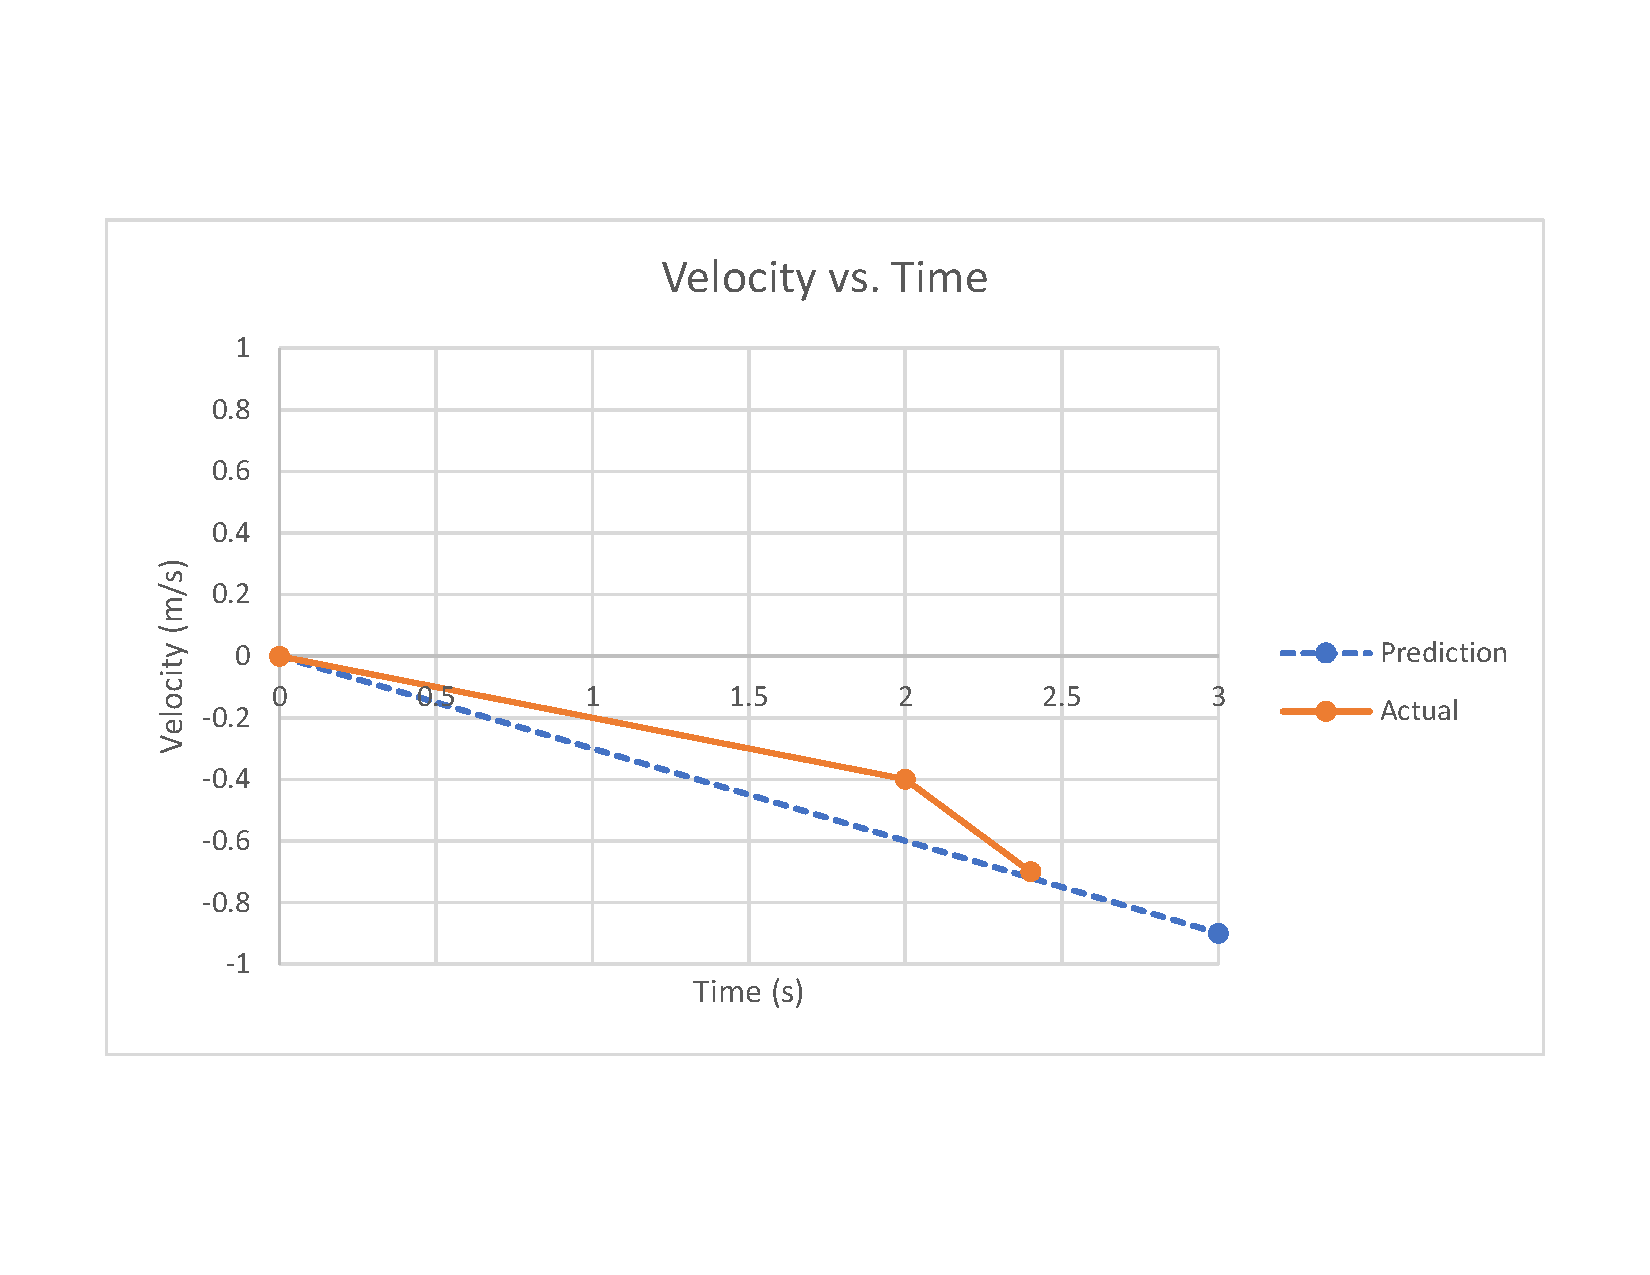
\includegraphics[width=4in]{PartCVelocity.pdf}\\
\vspace{-10mm}
\textit{Figure 9b: The Velocity vs. Time graph from the motion produced by the experiment in part C. The dashed line is my prediction, and the solid line is the actual result of the experiment.}
\end{center}

\newpage

As the cart was speeding up and moving towards the sensor, the velocity started at zero and had a negative linear slope until we stopped it from crashing into the sensor. Moving towards the origin prompts negative values, in the velocity vs. time graph. While the cart was speeding up when moving towards the origin, the acceleration was negative and pointing towards the origin. The acceleration is negative because it's the rate of change of velocity and the slope of the velocity graph was negative. 

\subsubsection{Constructing Acceleration Vectors for Speeding Up}

Just like in part A and part B, acceleration and velocity can be represented by vectors. In this case, the cart will start farthest away from the sensor and the velocity vectors are pointing towards the origin. Figure 10 show that the Magnitude of velocity is greater as time increases and the distance traveled in the interval of time is increased exponentially. 

\begin{center}
Figure 10\\
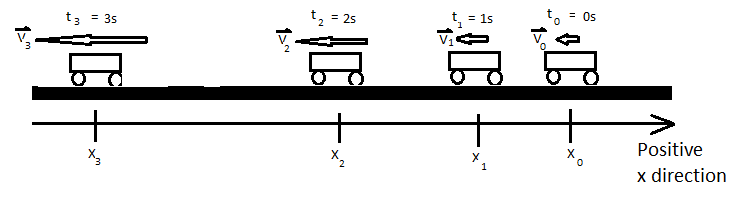
\includegraphics[width=4in]{VectorPartC.png}\\
\textit{Figure 10: Diagram that models the motion produced in part C, the velocity vectors on top of the cart show the approximate magnitude of velocity at the specific time.}
\end{center}

The acceleration vector between the times 1s and 2s in figure 10 can be produced by the equation, $\vec{a} = \frac{\vec{v_2} - \vec{v_1}}{t_2 - t_1}$. Since $|\vec{v_2}|$ is greater than $|\vec{v_1}|$, the acceleration vector will be negative and pointing towards the origin(left). The negative acceleration vector agrees with the acceleration vs. time graph(figure 9a) because they are both negative indicating that the acceleration is pointing towards the origin. 

\subsubsection{General Rule for Predicting Sign and Direction of Acceleration-Revisited}

The general rule that was made earlier was correct, but another point can be added. The velocity and acceleration would be negative if the vector is pointing towards the origin, and it would be positive if the vectors were pointing away from the origin.

\subsection{Toward the Detector and Slowing Down}

This section will be strictly analyzing the acceleration and velocity vectors created in an experiment that is moving towards the detector and slowing down. Figure 11 is the diagram of the experiment in this section, showing that the magnitude of the velocity vector is decreasing while moving towards the sensor. This distance being traveled over the interval of times is decreasing as the cart gets closer to the origin.

According to my general rule, the sign of acceleration would be positive, and the direction of the acceleration vector would be pointing away from the origin. The magnitude of the velocity vectors will become shorter and shorter as time increases, until the cart's velocity is zero and changes directions or until the cart crashes into the sensor with a lower velocity from when it started.  

\begin{center}
Figure 11\\
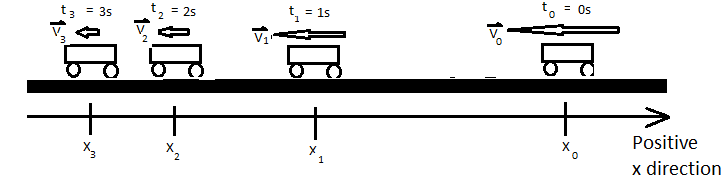
\includegraphics[width=4in]{VectorPartD.png}\\
\textit{Figure 11: Diagram that models the motion produced in part D, the velocity vectors on top of the cart show the approximate magnitude of velocity at the specific time.}
\end{center}

The acceleration vector can be found using the equation, $\vec{a} = \frac{\vec{v_2} - \vec{v_1}}{t_2 - t_1}$. Since $|\vec{v_1}|$ is greater than $|\vec{v_2}|$, the acceleration vector is point opposite of the direction of the velocity vectors. This acceleration vector would be pointing away from the origin and would be positive because it's pointing away from the origin. This acceleration vector agrees with the predictions made using my general rule.

\subsection{Reversing Direction}

In this final section, the motion being analyzed will be a cart moving away from the origin, but slowing down. The cart will slow down until it stops and changes directions, to start moving back towards the origin. The following data table is my prediction of the velocity and acceleration of the cart when it's moving away from the origin, turning around, and moving towards the origin.

\begin{center}
\begin{tabular}{|c|c|c|c|}
\hline
  & Moving Away & Turning Around & Moving Toward\\
\hline
Velocity: & Positive & Zero & Negative\\
\hline  
Acceleration: & Negative & Negative & Negative\\
\hline
\end{tabular}
\end{center} 

\newpage

Figure 12 shows my predictions(dashed lines) and actual data(solid lines) from the acceleration vs. time and velocity vs. time graphs representing motion away from the origin, slowing down and turning around, and coming back towards the origin with increasing speed. 

\begin{center}
Figure 12\\
\vspace{-10mm}
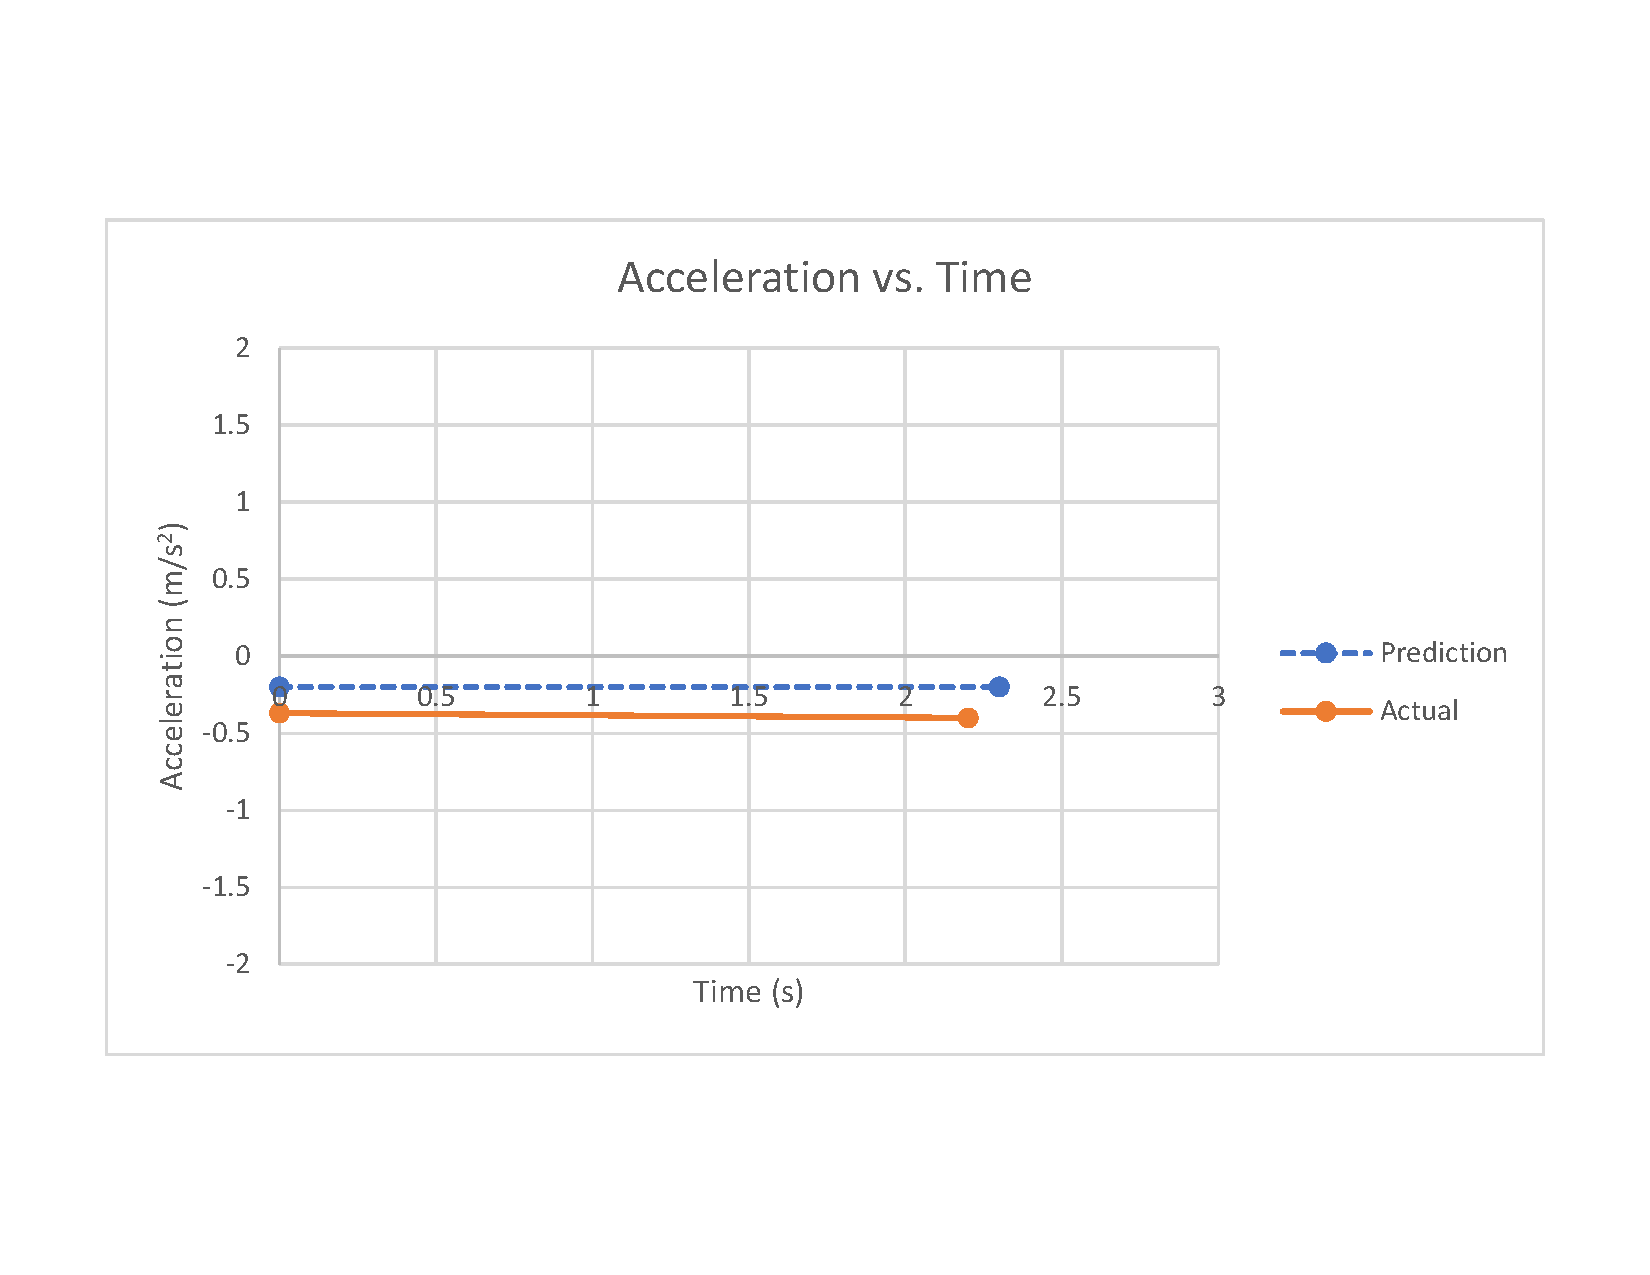
\includegraphics[width=4in]{PartEAcceleration.pdf}\\
\vspace{-10mm}
\textit{Figure 12a: The Acceleration vs. Time graph from the motion produced from movement away from the origin and then turning around and moving back towards the origin. The dashed line is my prediction of the experiment, and the solid line is the actual result of the experiment.}\\
\vspace{10mm}
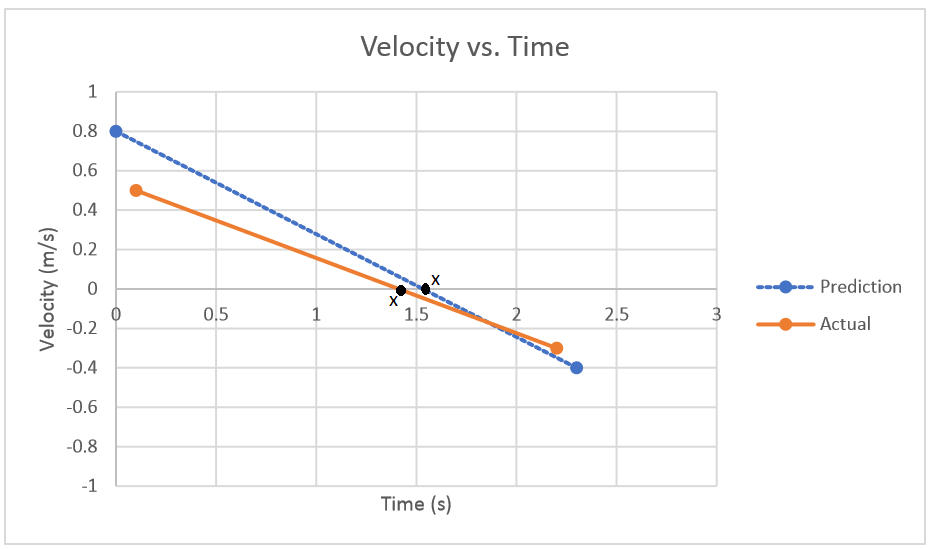
\includegraphics[width=4in]{PartEVelocity.png}\\
\textit{Figure 12b: The Velocity vs. Time graph from the motion produced by the experiment. The dashed line is my prediction, and the solid line is the actual result of the experiment.}
\end{center}

The cart reaches it's farthest distance when the velocity is zero on the velocity graph. The farthest distance is denoted by an "X" on the line which can be seen when the velocity value is at zero. The velocity at the moment it switches direcions is zero, this agrees with my prediction. The acceleration at the instant it is turning around was $\approx -0.4 \frac{m}{s^2}$, this does agree with my prediction except I thought the value would be closer to the x-axis. The acceleration throughout the system was negative. Since the velocity graph had a linear line, sloping downward, the slope indicates that the acceleration was negative. The velocity at the moment after it's zero and turning around would be negative because it's now moving towards the origin. It makes sense because the acceleration is negative, so at some time it can be predicted that the velocity go from positive to zero and from zero to negative, indicating that the cart is turning around and moving towards the origin. 

\subsubsection{General Rule for Predicting the Sign and Direction of Acceleration-Revisted One Last Time}

My General rule from earlier was correct. When moving towards the origin, velocity had a negative sign. When moving away from the origin, velocity has a positive sign. When the cart is moving away from the origin and speeding up, the acceleration is positive. When the cart is moving away from the origin and slowing down, the acceleration is negative. When the cart is moving towards the origin and speeding up, the acceleration is negative. When the cart is moving towards the sensor and slowing down, the acceleration is positive. Positive values are produced when the vectors are pointing away from the origin and negative values are produced when the vectors are pointing towards the origin.


\section{Discussion} 

The one dimensional kinematic systems that were analyzed in the experiment are all governed by classical mechanics. When looking at the slope of the velocity graph, it was possible to analyze acceleration. During the experiment, it was exciting to see the intimate relationship between the mathematical, graphical, and physical representation of the one dimensional kinematic systems. The mathematical $\frac{dv}{dt}$ was seen in the velocity graphs by looking at the slopes, and represented physically through the speeding up or slowing down of the cart on the "frictionless" track. To understand the concepts in this experiment well, it is essential to understand that all motion is in respect to an origin.  



\section{References}

\hspace{-6.5mm}
Introduction to Motion II Physics 06 Lab, Dr. Melanie Lutz\\



\end{document}
